\documentclass{article}
\usepackage{graphicx}
\usepackage[table,xcdraw]{xcolor}
% \graphicspath{ {./Pictures/} }
\usepackage{float}
\begin{document}
\subsection{Transakcije}
\subsubsection{M-banking}

\textbf{Slučaj upotrebe: M-banking (Internet plaćanje):}
\begin{enumerate}
  \item \textbf{Kratak opis: }
  Beskontaktno plaćanje dobara ili usluga.
  \item \textbf{Učesnici: }
    \begin{itemize}
        \item Kupac - želi brzu i efikasnu uslugu
        \item Eksterni sistem davaoca usluge ili dobra
     \end{itemize}
  \item \textbf{Preduslovi: }
    Kupac ima aktivan račun u sistemu banke, davalac usluge ima aktivan račun u nekoj od banaka, davalac usluge ili dobra ima omogućeno internet plaćanje.
  \item \textbf{Postuslovi: }
    Transakcija je ispravno izvršena, sredstva sa računa kupca su prebačena na račun davaoca usluge ili dobra.
  \item \textbf{Osnovni tok: }
    \begin{enumerate}
        \item Korisnik se povezuje na sajt davaoca usluge ili dobra
        \item Korisnik bira artikle koje želi da kupi i stavlja ih u korpu
        \item Korisnik završava izbor artikala i prelazi na izvršavanje kupovine
        \item Korisnik popunjava formular sa podacima vezanim za izvršavanje kupovine (lične podatke korisnika, adresu dostavljanja dobra ili izvršenje usluge, kontakt telefon, kontakt mejl)
        \item Eksterni sistem davaoca usluge ili dobra proverava da li su sva obavezna polja popunjena i ispunjeni uslovi datih polja
        \item Korisnik popunjava podatke za plaćanje (broj kartice i sigurnosni kod, kao i kod sigurnosne provere, captcha)
        \item Eksterni sistem davaoca usluge ili dobra šalje validacioni kod korisniku putem sms poruke
        \item Korisnik prima i unosi validacioni kod u predviđeno polje
        \item Eksterni sistem davaoca usluge ili dobra proverava validnost unesenog koda
        \item Eksterni sistem davaoca usluge šalje zahtev sistemu banke za transakciju zajedno sa podacima plaćanja (broj kartice i sigurnosni kod)
        \item Sistem banke prima zahtev za transakciju i proverava podatke plaćanja
        \item Sistem banke proverava mogućnost izvršavanja transakcije (da li kupac ima dovoljno sredstava na računu)
        \item Sistem banke skida sredstva sa računa kupca i šalje na račun davaoca usluge ili dobra
        \item Sistem banke šalje odgovor eksternom sistemu o izvršavanju transakcije
        \item Eksterni sistem obaveštava kupca o izvršenju procesa kupovine usluge ili dobra
    \end{enumerate}
  \item \textbf{Podtokovi: } /
  \item \textbf{Alternativni tokovi: }
    \begin{enumerate}
        \item \textbf{Nevalidno popunjena polja formulara sa podacima: } Korisnik nije uneo ime ili prezime, ili je uneo nevalidan format mejla u koraku d, isti se obaveštava da iste mora popuniti na validan način.
        \item \textbf{Nevalidno popunjena captcha: } Korisnik nije uneo validan sigurnosni kod u koraku e, isti se obaveštava da sigurnosni kod mora da se poklapa i šalje mu se novi koji treba uneti.
        \item \textbf{Korisniku nije stigao validacioni kod: } Ukoliko korisniku nije stigao validacioni kod od strane eksternog sistema, u koraku g, korisnik može zatražiti novi kod.
        \item \textbf{Sistem banke primio nevalidne podatke transakcije: } Ukoliko sistem banke obavesti eksterni sistem o nevalidnosti transakcije vezane za broj kartice i sigurnosni kod; korisnik dobija informaciju o neuspehu i mora ponoviti kupovinu od početka ukoliko želi da je izvrši.
        \item \textbf{Sistem banke pri proveri stanja utvrđuje da transakcija zahteva više sredstava nego što je na računu: } Ukoliko sistem banke obavesti eksterni sistem o manjku sredstava: korisnik dobija informaciju o 
        manjku sredstava i kupovina mu se poništava.
    \end{enumerate}
  \item \textbf{Specijalni zahtevi: } Korisnik mora imati telefon sa povezanim brojem na račun u sistemu banke.
  \item \textbf{Dodatne informacije: } /
\end{enumerate}

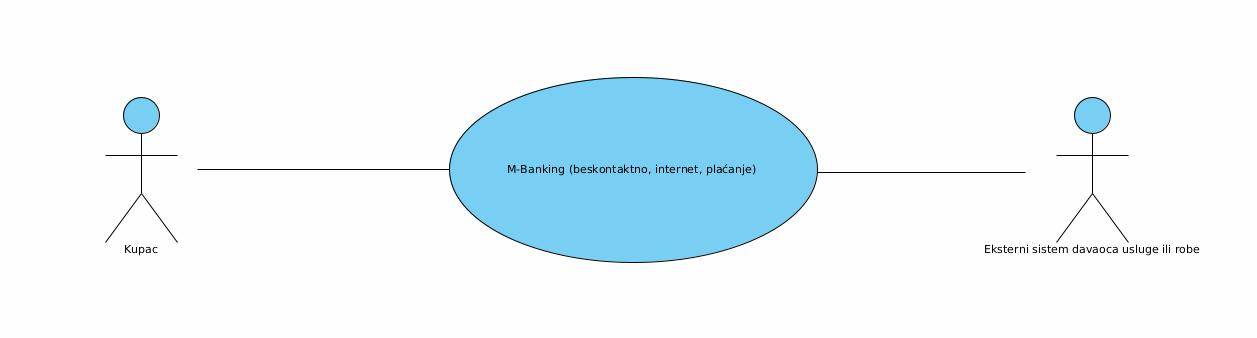
\includegraphics[scale = 0.27]{./UseCases/Pictures/M-Banking.jpg}


\end{document}
